\section{Preliminary Work}\label{preliminary}


Conclusion is finding the right approach to deployment and what sort of gases should I measure and the platform I should use (how can I engineer a platform based on this device)

During the course of working on the MPP and MPP1 reports, preliminary work was carried out in order to efficiently form a work plan. In this preliminary work the challenges which would be faced were identified, as well as a background report on the definition of \emph{air quality}, the creation of heat maps, which are the standard representation format for display air quality information \todo{CITE ME}. Finally some research was carried out into building an appropriate sensor platform.


\subsection{Challenge Identification}\label{challenges}

In order to effectively evaluate the task at hand the challenges involved must first be identified. With regards to this the following challenges were identified as being the most important overall aims for the project, at least in the current stage. 

\begin{itemize}
	\item What to measure?

	In order to measure air quality effectively a standard definition should be used. Research showed that there was very little consensus on the definition of air quality and so a definition which this thesis will use as the standard must be defined. The definition must also include a list of chemicals so that the appropriate hardware can be used to generate readings. This ensures that the solution is also cost effective. 

	\item Deployment considerations

	In the MInf Project Proposal stage it was discovered that there are certain considerations which must be made in order to effectively measure air quality. As can be seen in Figure~\ref{fig:stationarypollutantbuildup}, which shows the initial motion of a bus with an air quality sensor on the top deck, pollutants build up when the bus is stationary and only disperse after a certain amount of time which is dependent on the current weather and motion of the bus.

	\begin{figure}[H]
        \begin{center}
                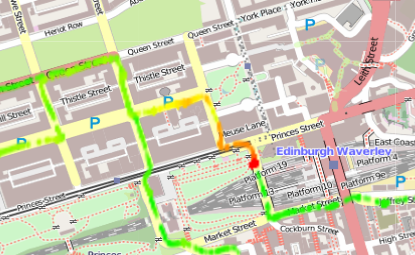
\includegraphics[scale=0.8]{./images/mpp1/StationaryPollutantBuildUp.png} 
                \caption{Example of pollutant build up in stationary situations. In this example the bus starts where the highest concentration of pollutants is found, denoted by the red, and moves in a northern direction initially.}
                \label{fig:stationarypollutantbuildup}
        \end{center}
	\end{figure}

	It was also found that certain measurements were dependant on other factors. Temperature, for instance, was dependant on the direction of the bus due to the sensors location at the back. When the bus turned towards the south, the sunlight hit the temperature sensor directly which caused a spike in temperature readings. Humidity showed a similar response to the air pollutants. 

	With regards to this it has been determined that in order to continue with the original plan of mounting the sensors on buses, a suitable enclosure must be designed which will remove direct sunlight and build up of pollutants from the data. It may be that it is not possible to remove the pollutant build up and stops may need to be recorded so that the data can be corrected for this discrepancy, whether by adjusting the recorded values automatically, or simply removing it from the data set. 

	\item Calibration

	Each sensor is different from other models and even subtly different from other samples of the same model. In order to compensate for this calibration must be performed. In certain situations it may be sufficient to simply measure against a baseline before starting the data collection, however in others calibration may be needed periodically. 

	Projects such as the OpenSense deployment in Zurich~\cite{opensensezurich} perform periodic calibrations when the trams come within a certain distance of each other. 


	\item Data collection
	
	Data collection is the main goal of this project. The aim of this is to have a method which is both efficient, in terms of power consumption and reliability, and responsive. In order to do this there are multiple methods of uploading data which can be trialled to find that which is the most effective.

	\item Interpolating and extrapolation

	When dealing with a data set such as air quality readings where we only have sparse data measurements it is important to represent the data as clearly as possible. In order to do this a method of interpolation, and potentially extrapolation, must be employed. Multiple different models will be evaluated and compared in order to select the model which is most appropriate for generating the expected output.

\end{itemize}



\subsection{Air Quality}\label{airquality}

\subsubsection{Definition}\label{airqualitydefinition}

A definition of air quality is a difficult problem which has not been solved. Many institutions measure and record what they refer to as ``air quality'', however the only thing these measurements have in common is that no two are the same. In order to research the area of ``air quality'' further we must have a concrete definition of what air quality is. Current definitions give a simple definition of ``air quality'' as being antonymous to that of air pollution in that higher air quality is the equivalent to low air pollution\cite{bcaq}. This implies that not only should the metrics used for defining air quality be considered, but also those used to define air pollution.

Looking at statements and measurements by various authorities around the world \cite{epapollutants}\cite{airqualityobjectives}\cite{cleanairnavigation}\cite{naaqs}\cite{whoguidelines}, we can build a list of common pollutants which are measured:


\begin{itemize}
\item Sulphur dioxide
\item Nitrogen dioxide
\item PM10 
\item PM2.5
\end{itemize}

These chemicals can form the basis of pollutants which in turn can help define ``air quality''. By looking at other sources\cite{meaningsofenvironmentalterms},  proposed definition of ``air quality'' is as follows:

\begin{quote}
``The current measurements of the concentrations of certain pollutants in the air relative to the requirements of one or more biotic species or to any human need or purpose.''
\end{quote}

\subsubsection{Measurement}\label{airqualitymeasurement}

\paragraph{Sensors and Calibration} \hspace{0pt} \\

In order to measure pollutants and other factors relating to air quality we rely on electrochemical, solid state, or mechanical sensors, with the former being the most popular. The nature of sensors presents some unique problems. Mechanical sensors, such as those used for measuring pressure, may seize up and provide inaccurate measurements. Electrochemical sensors, which use an active surface, decay over time. This project will be using electrochemical sensors only, and so only suffers from the latter problem. 

\emph{How Electrochemical Sensors Work}

An electrochemical sensor is made up of the following components:\cite{intlelectrochemicalsensor}

\begin{itemize}
	\item Anode
	\item Cathode
	\item Gas Permeable Membrane % - This covers the electrode in the sensor from contamination, while still allowing gases to pass though.
	\item Electrolyte % - Something about reactions...
\end{itemize}

By reacting the target gas at the anode and measuring the resulting current generated we can calculate how much of the target gas is present. In sensors which react with the target gas at the anode, oxygen is needed at the cathode as can be seen from the following chemical reactions.

At anode:

\begin{align*}
	\cee{\emph{Carbon Monoxide: } CO + H_{2}O &-> CO_{2} + 2H+ 2e- \\
	\\
	\emph{Hydrogen Sulphide: } H_{2}S + 4H_{2}O &-> H_{2}SO_{4} + 8H+ + 8e- \\
	\\
	\emph{Nitrous Oxide: } NO + 2H_{2}O &-> HNO_{3} + 3H+ + e- \\
	\\
	\emph{Hydrogen Cyanide: } 2HCN + Au &-> HAu(CN)_{2} + H+ + e-}
\end{align*}
At cathode:
\begin{align*}
	\cee{O_{2} + 4H+ + 4e- &-> 2H_{2}O \\}
\end{align*}

Insufficient oxygen at the cathode causes the cathode to degrade resulting in changing readings. 

In other types of sensors, which react with the target at the cathode, oxygen is not always necessary. For example:

\begin{align*}
	\cee{\emph{Nitrous Oxide: } NO_{2} + 2H+ + 2e- &-> NO + H_{2}O \\
	\\
	\emph{Chlorine: } Cl_{2} + 2H+ + 2e- &->  2HCl\\
	\\
	\emph{Ozone: } O_{3} + 2H+ + 2e- &-> O_{2} + H_{2}O }
\end{align*}

While oxygen is not a requirement, these sensors do eventually degrade due to the fact that no chemical reaction is going to be 100\% efficient.

\emph{Solid State Sensors}

I'm pretty sure the sensors I have are electrochemical so I haven't read much about this yet, but I will have 

\emph{Calibration}

In order to continue using sensors as they degrade, they must be calibrated regularly. The most simple method of calibration, employed by projects such as OpenSense, simply use a known reliable sensor to take readings at the same point of space and time and calibrated using this data as a reference.






\subsection{Heat maps}\label{heatmaps}


\subsubsection{Definition}\label{heatmapdefinition}

A heat map is a two dimensional graphical representation of a matrix using colours to correspond to different magnitudes of values. It is a thematic map of a matrix, although can also be applied to geographical maps. 

\begin{figure}[H]
        \begin{center}
                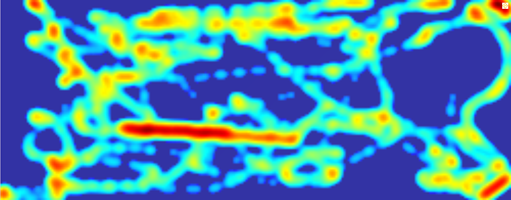
\includegraphics[scale=0.5]{./images/heatmaps/ExampleMouseMove.png}
                \caption{Example heat map generated from mouse movements}
                \label{fig:mousemoveheatmap}
        \end{center}
\end{figure}

Heat maps are generally used to quickly display which values in a matrix have the greatest magnitude and how they compare to surrounding values. Figure~\ref{fig:mousemoveheatmap}, which represents mouse movements on a website clearly shows a horizontal band in the middle which indicates that the users mouse spent a lot of time there. 

\paragraph{Calculations and Colour Progression} \hspace{0pt} \\


In order to create an image representation of the matrix, a colour progression must be chosen. The simplest colour progression method is a hue change on a single colour corresponding to the information. However this may not always be the most suitable method. When giving out information to the public, certain colours tend to represent different things. Red normally has negative connotations while green is the opposite. For this we can use a blended hue colour progression with red at one end of the scale and green at the other.


\paragraph{Representation Matrix} \hspace{0pt} \\

In order to generate the heat map we first need a matrix. A simple matrix can generate an effective heat map as can be seen from the following example.

\begin{figure}[H]
        \begin{center}
                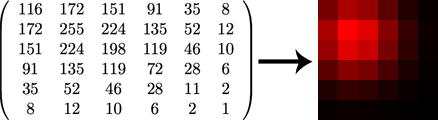
\includegraphics[scale=0.5]{./images/heatmaps/HeatMapGaussianExample.png}
                \caption{Heat Map Generation Example}
                \label{fig:matrixheatmapexample}
        \end{center}
\end{figure}

The example in figure~\ref{fig:matrixheatmapexample} has the maximum value of 255 represented by red (RGB value of \#FF0000) and the minimum value of 1 being almost black (RGB value \#010000). 

\emph{Missing Values}

With many applications there are either missing values in the matrix, or the values cannot be easily placed into a matrix (as is the case for geographical readings). To find the missing values, interpolation of some kind is used. In figure~\ref{fig:matrixheatmapexample} the matrix was generated by placing the value 255 in position (2,2) and performing a Gaussian blur with a filter size of 2 by 2 pixels and sigma equal to 2. 

Irregular data points must be processed further by mapping them onto a matrix. In the case of taking geographical readings, the heat map can be regenerated for each zoom level to ensure the maximum accuracy. 

These methods are not completely accurate and the missing data should be calculated in a manner appropriate to the application.

\subsubsection{Applications in Air Quality Measurement}\label{applicationsinaqmeasurement}

Heat maps are extremely useful to show the concentrations of pollutants in geographical areas. The information is easily given when overlaid on top of a map.  

\begin{figure}[H]
        \begin{center}
                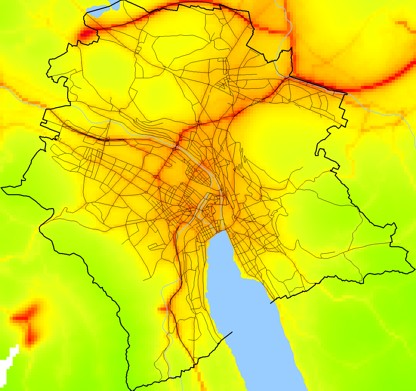
\includegraphics[scale=0.5]{./images/heatmaps/zurichpm.jpg}
                \caption{Particulate matter heat map in Zurich. Source: \url{www.stadt-zuerich.ch}}
                \label{fig:pmheatmapzurich}
        \end{center}
\end{figure}

From the above image we an easily see that the highest concentrations of particulate matter are where the roads are situated indicating a relationship between the two. 






\subsection{Sensor Creation}\label{Sensor Creation}






